%!TEX root = ../thesis.tex
%*******************************************************************************
%****************************** Third Chapter **********************************
%*******************************************************************************
\chapter{Experiments}

% **************************** Define Graphics Path **************************
\ifpdf
    \graphicspath{{Chapter3/Figs/Raster/}{Chapter3/Figs/PDF/}{Chapter3/Figs/}}
\else
    \graphicspath{{Chapter3/Figs/Vector/}{Chapter3/Figs/}}
\fi

We compare the accuracy of gMatrix without partitioning and with partitioning for answering edge frequency estimation querie

\section{System Description}
The code is implemented in C++ and experiments were performed on Intel Xeon 2GHz 16GB server.

\section{Datasets}
The datasets used to evaluate the sketches are graph streams consisting of distinct edges only. The datasets are:
\begin{itemize}
\item IP-Trace Network Stream \cite{khan}
\item Twitter Communication Stream \cite{khan}
\item Friendster Stream with Zipf Frequency distribution \cite{khan}
\end{itemize}

\section{Metrics}
\subparagraph{Observed Error \cite{khan}}
\[
observed\;error = \frac{ \sum_{i=1}^{|Q|}{|\tilde{f}(q_i) - f(q_i)|} }{\sum_{i=1}^{|Q|}f(q_i)}
\]
where $Q = \{q_i\}$ is the set of queries, $\tilde{f}$ is the estimated frequency, and $f$ is the actual frequency.

\subsection{Average Relative Error \cite{DBLP}}
\[
average\;relative\;error = \frac{1}{|Q|} \sum_{i=1}^{|Q|} \frac{\tilde{f}(q_i)-f(q_i)}{f(q_i)}
\]
where $Q = \{q_i\}$ is the set of queries, $\tilde{f}$ is the estimated frequency, and $f$ is the actual frequency.

\subsection{Effective Queries \cite{DBLP}}
Both Observed Error and Average Relative Error may be biased if the frequencies of the queries vary a lot, so we define queries as "effective" if the relative error is not exceeding $G_0$. The percentage of effective queries is computed by,
\[
effective\;queries = \frac{|\{q|\frac{\tilde{f}(q)-f(q)}{f(q)} \leq T, q \in Q\}|}{|Q|} \cdot 100\%
\]
where $Q = \{q_i\}$ is the set of queries, $\tilde{f}$ is the estimated frequency, and $f$ is the actual frequency.

In this experiment, $T$ is set to 5, which is the same as \cite{DBLP}.


\section{Results}
The results of the experiment are shown in Figures \ref{fig:f1}, \ref{fig:f2}, \ref{fig:f3}, \ref{fig:t1}, \ref{fig:t2}, \ref{fig:t3}, \ref{fig:i1}, \ref{fig:i2}, and \ref{fig:i3}.

\begin{figure}[!htbp]
\centering
\begin{subfigure}{.5\textwidth}
  \centering
  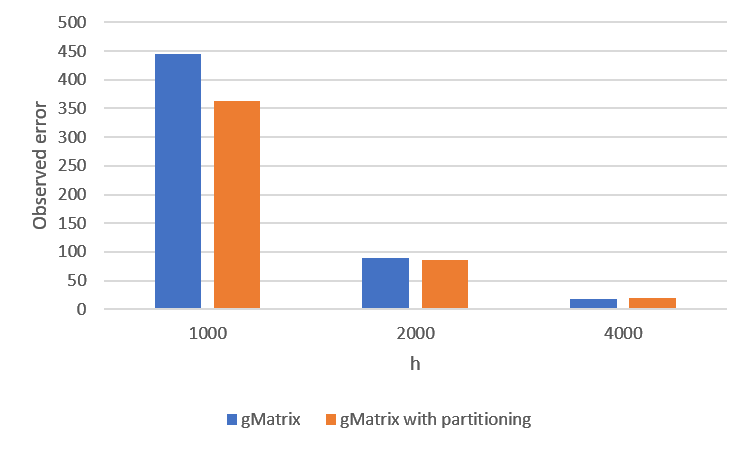
\includegraphics[width=1\linewidth]{F1}
  \caption{w = 10, outlier partition = 17\%}
  \label{fig:sub1}
\end{subfigure}%
\begin{subfigure}{.5\textwidth}
  \centering
  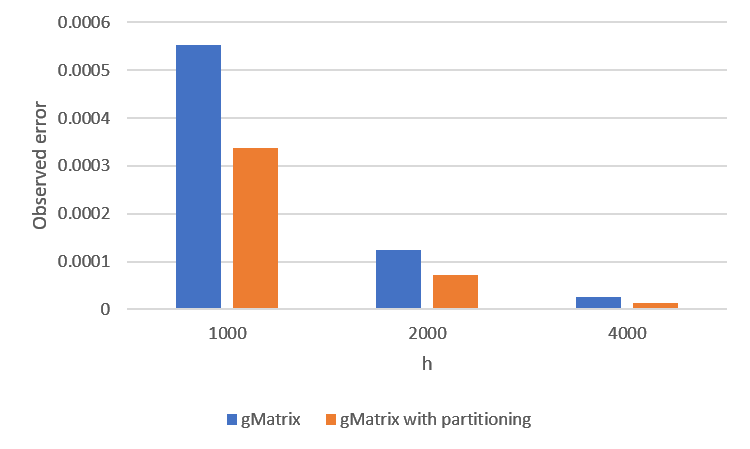
\includegraphics[width=1\linewidth]{F1T}
  \caption{w = 10, outlier partition = 17\%}
  \label{fig:sub2}
\end{subfigure}
\caption{Observed error of Friendster dataset considered over (a) 1 million random edges and (b) top 500 highest frequency edges.}
\label{fig:f1}
\end{figure}

\begin{figure}[!htbp]
\centering
\begin{subfigure}{.5\textwidth}
  \centering
  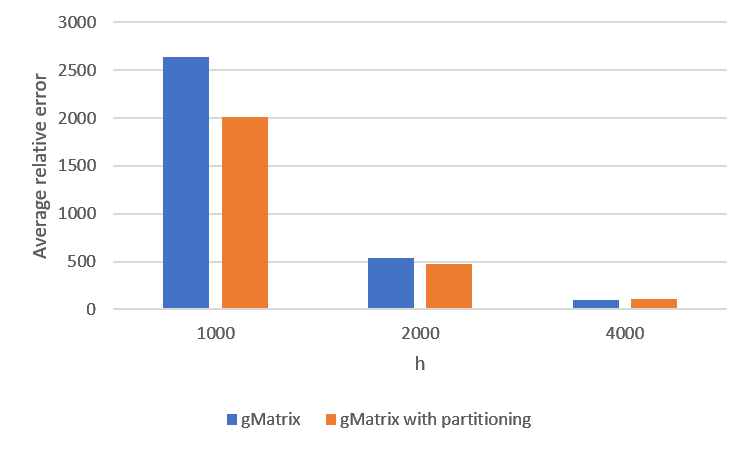
\includegraphics[width=1\linewidth]{F2}
  \caption{w = 10, outlier partition = 17\%}
  \label{fig:sub1}
\end{subfigure}%
\begin{subfigure}{.5\textwidth}
  \centering
  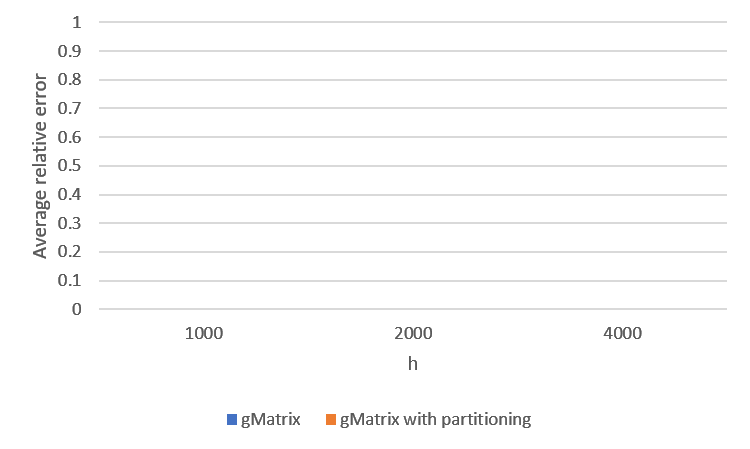
\includegraphics[width=1\linewidth]{F2T}
  \caption{w = 10, outlier partition = 17\%}
  \label{fig:sub2}
\end{subfigure}
\caption{Average relative error of Friendster dataset considered over (a) 1 million random edges and (b) top 500 highest frequency edges.}
\label{fig:f2}
\end{figure}

\begin{figure}[!htbp]
\centering
\begin{subfigure}{.5\textwidth}
  \centering
  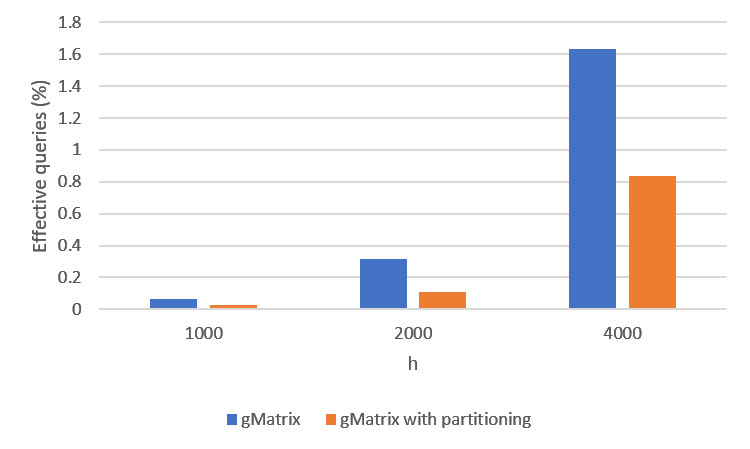
\includegraphics[width=1\linewidth]{F3}
  \caption{w = 10, outlier partition = 17\%}
  \label{fig:sub1}
\end{subfigure}%
\begin{subfigure}{.5\textwidth}
  \centering
  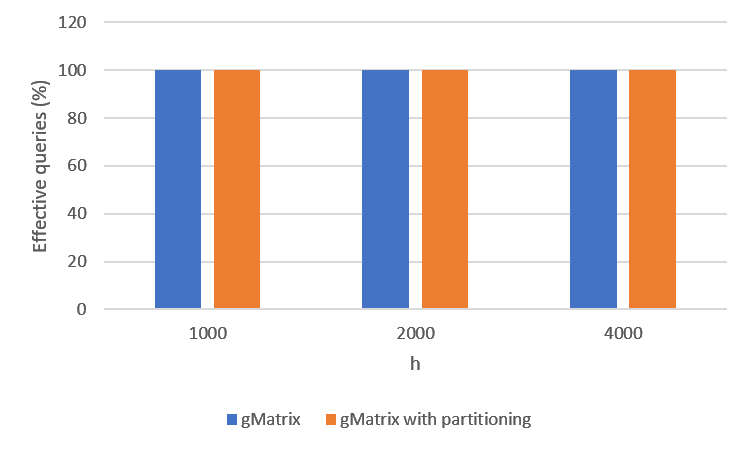
\includegraphics[width=1\linewidth]{F3T}
  \caption{w = 10, outlier partition = 17\%}
  \label{fig:sub2}
\end{subfigure}
\caption{Percentage of effective queries of Friendster dataset considered over (a) 1 million random edges and (b) top 500 highest frequency edges.}
\label{fig:f3}
\end{figure}

\begin{figure}[!htbp]
\centering
\begin{subfigure}{.5\textwidth}
  \centering
  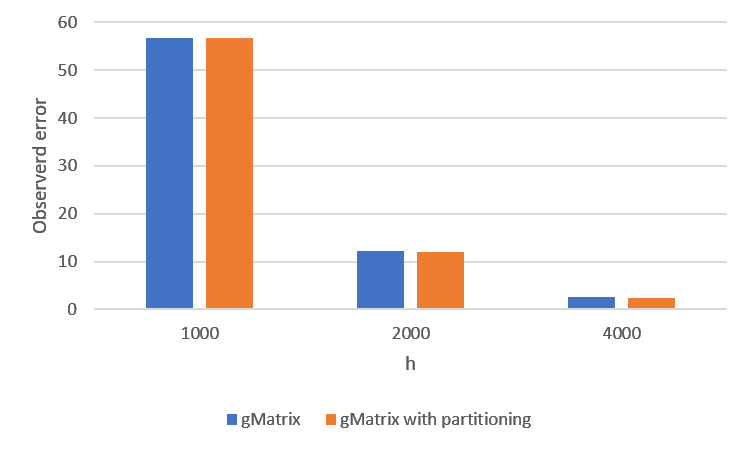
\includegraphics[width=1\linewidth]{T1}
  \caption{w = 10, outlier partition = 23\%}
  \label{fig:sub1}
\end{subfigure}%
\begin{subfigure}{.5\textwidth}
  \centering
  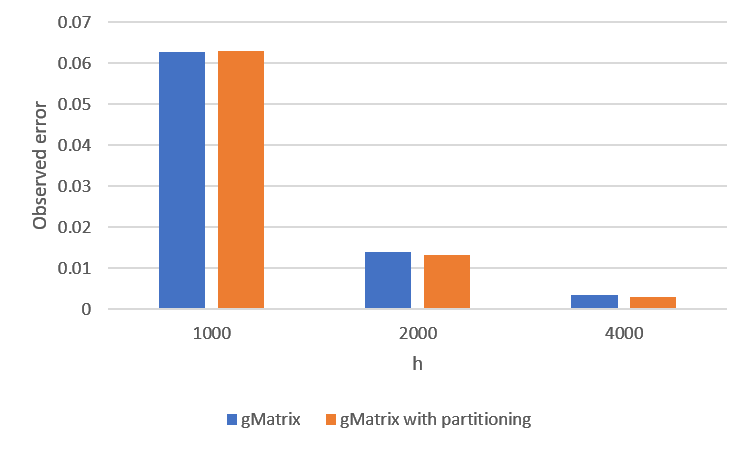
\includegraphics[width=1\linewidth]{T1T}
  \caption{w = 10, outlier partition = 23\%}
  \label{fig:sub2}
\end{subfigure}
\caption{Observed error of Twitter dataset considered over (a) 1 million random edges and (b) top 500 highest frequency edges.}
\label{fig:t1}
\end{figure}

\begin{figure}[!htbp]
\centering
\begin{subfigure}{.5\textwidth}
  \centering
  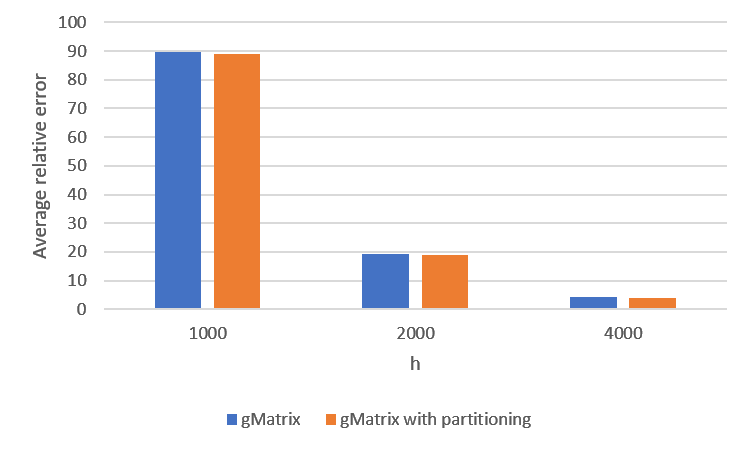
\includegraphics[width=1\linewidth]{T2}
  \caption{w = 10, outlier partition = 23\%}
  \label{fig:sub1}
\end{subfigure}%
\begin{subfigure}{.5\textwidth}
  \centering
  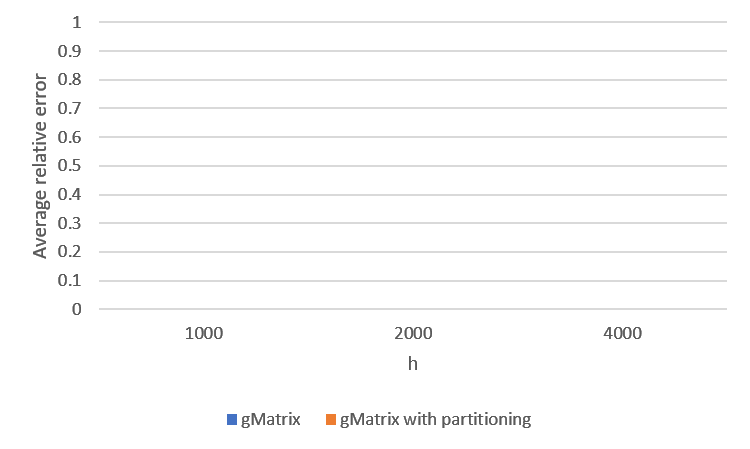
\includegraphics[width=1\linewidth]{T2T}
  \caption{w = 10, outlier partition = 23\%}
  \label{fig:sub2}
\end{subfigure}
\caption{Average relative error of Twitter dataset considered over (a) 1 million random edges and (b) top 500 highest frequency edges.}
\label{fig:t2}
\end{figure}

\begin{figure}[!htbp]
\centering
\begin{subfigure}{.5\textwidth}
  \centering
  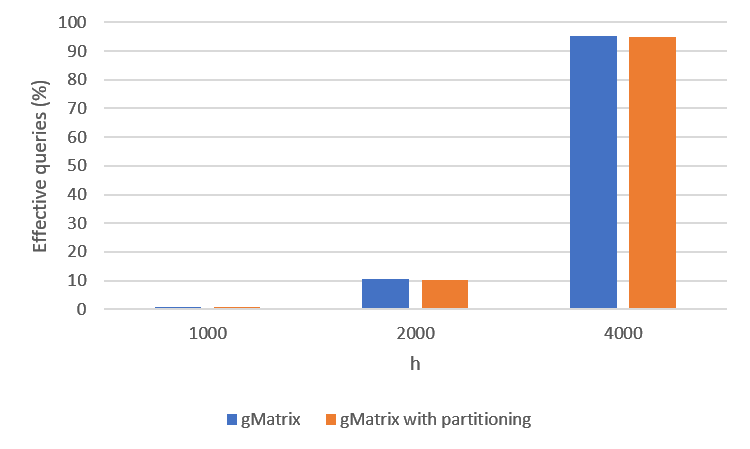
\includegraphics[width=1\linewidth]{T3}
  \caption{w = 10, outlier partition = 23\%}
  \label{fig:sub1}
\end{subfigure}%
\begin{subfigure}{.5\textwidth}
  \centering
  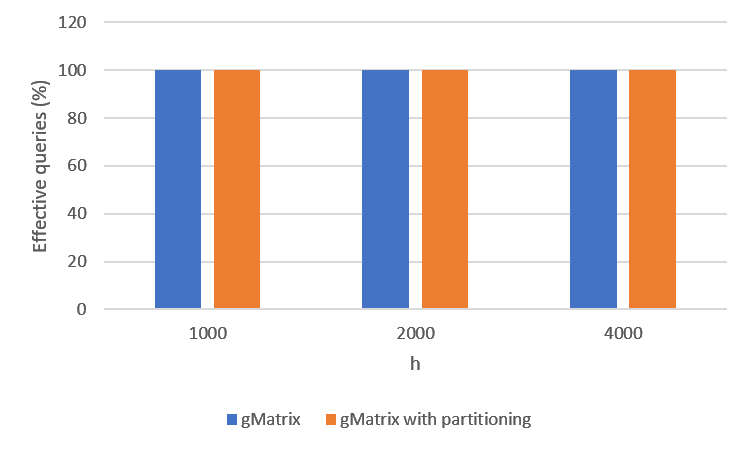
\includegraphics[width=1\linewidth]{T3T}
  \caption{w = 10, outlier partition = 23\%}
  \label{fig:sub2}
\end{subfigure}
\caption{Percentage of effective queries of Twitter dataset considered over (a) 1 million random edges and (b) top 500 highest frequency edges.}
\label{fig:t3}
\end{figure}

\begin{figure}[!htbp]
\centering
\begin{subfigure}{.5\textwidth}
  \centering
  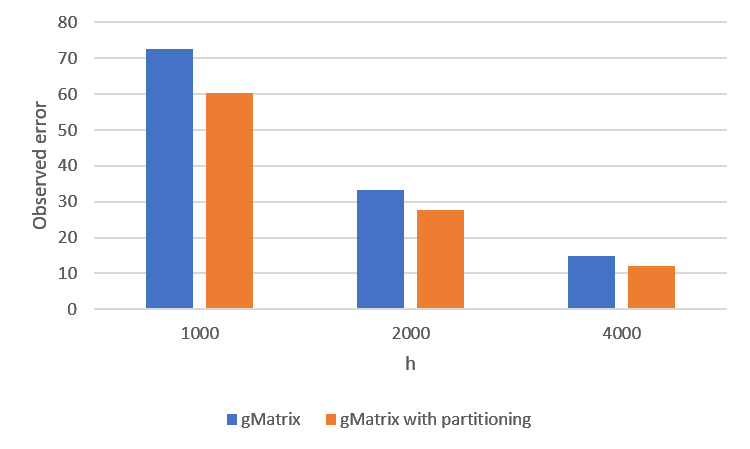
\includegraphics[width=1\linewidth]{I1}
  \caption{w = 10, outlier partition = 76\%}
  \label{fig:sub1}
\end{subfigure}%
\begin{subfigure}{.5\textwidth}
  \centering
  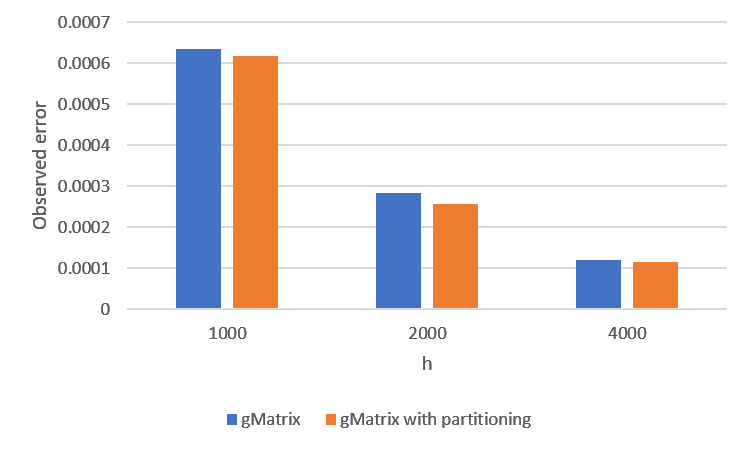
\includegraphics[width=1\linewidth]{I1T}
  \caption{w = 10, outlier partition = 76\%}
  \label{fig:sub2}
\end{subfigure}
\caption{Observed error of IP Trace dataset considered over (a) 1 million random edges and (b) top 500 highest frequency edges.}
\label{fig:i1}
\end{figure}

\begin{figure}[!htbp]
\centering
\begin{subfigure}{.5\textwidth}
  \centering
  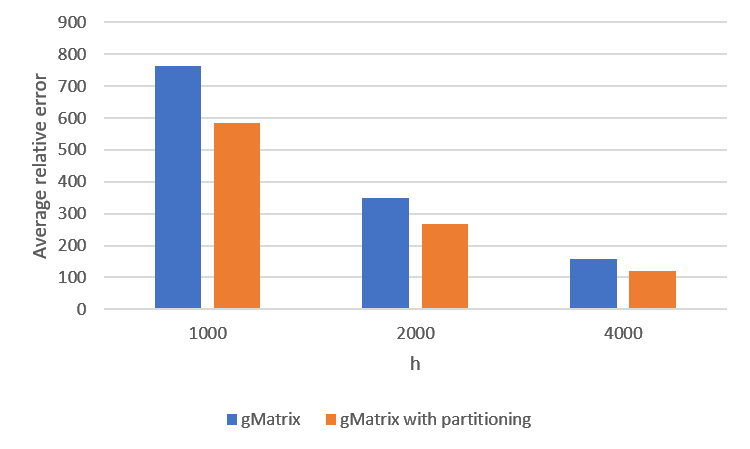
\includegraphics[width=1\linewidth]{I2}
  \caption{w = 10, outlier partition = 76\%}
  \label{fig:sub1}
\end{subfigure}%
\begin{subfigure}{.5\textwidth}
  \centering
  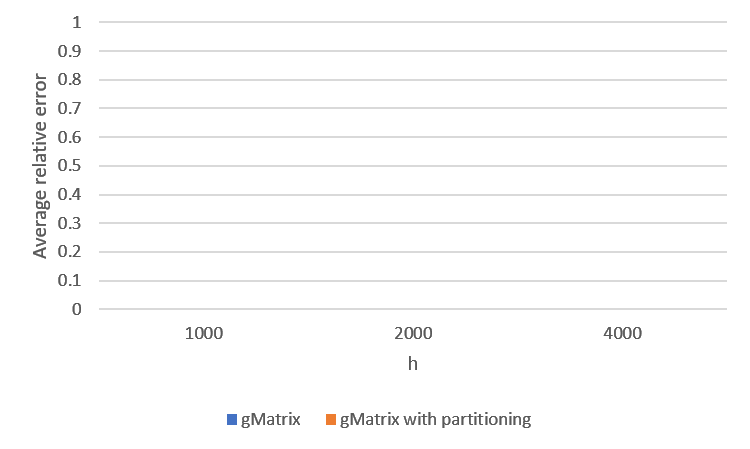
\includegraphics[width=1\linewidth]{I2T}
  \caption{w = 10, outlier partition = 76\%}
  \label{fig:sub2}
\end{subfigure}
\caption{Average relative error of IP Trace dataset considered over (a) 1 million random edges and (b) top 500 highest frequency edges.}
\label{fig:i2}
\end{figure}


\begin{figure}[!htbp]
\centering
\begin{subfigure}{.5\textwidth}
  \centering
  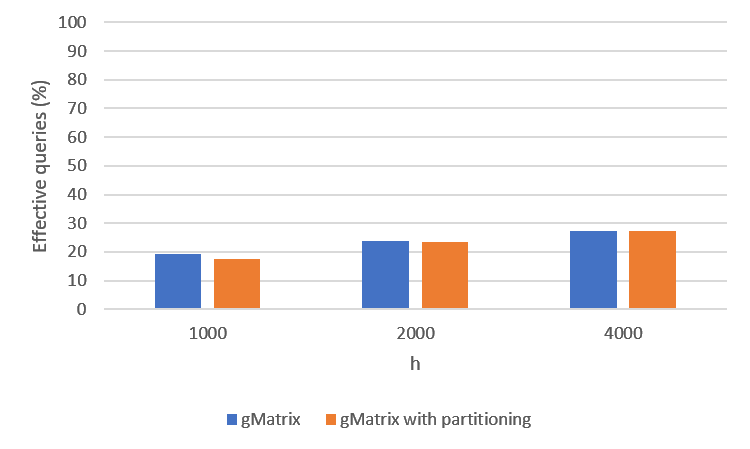
\includegraphics[width=1\linewidth]{I3}
  \caption{w = 10, outlier partition = 76\%}
  \label{fig:sub1}
\end{subfigure}%
\begin{subfigure}{.5\textwidth}
  \centering
  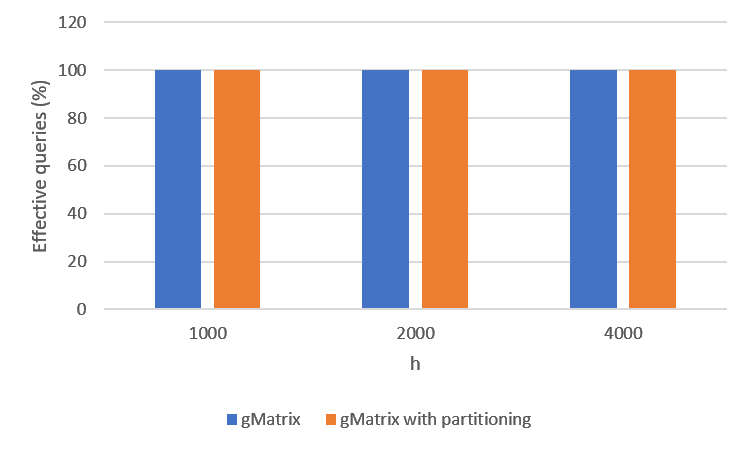
\includegraphics[width=1\linewidth]{I3T}
  \caption{w = 10, outlier partition = 76\%}
  \label{fig:sub2}
\end{subfigure}
\caption{Percentage of effective queries of IP Trace dataset considered over (a) 1 million random edges and (b) top 500 highest frequency edges.}
\label{fig:i3}
\end{figure}
